\section{Dissipation\label{sec:linbland1}}
In this chapter we will ultimately  look to understand the image below,
which  describes the  dissipation processes  that  can occur  in a  two
levels system

\begin{figure}[h]
  \centering 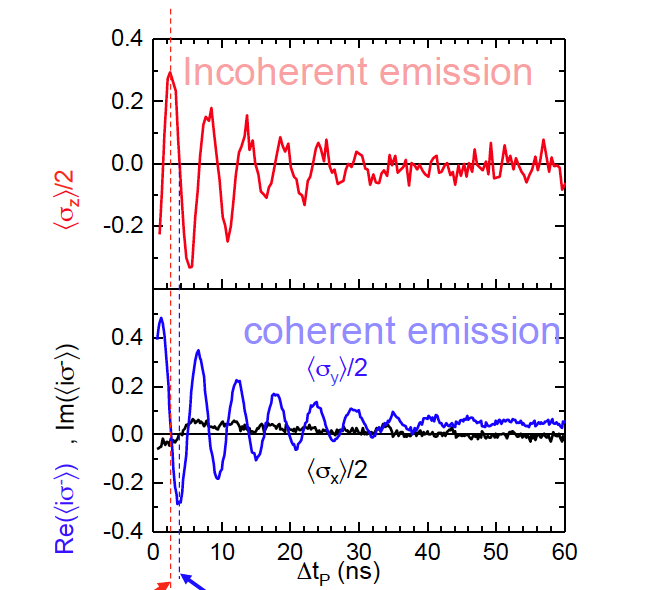
\includegraphics[height=5cm]{cohereneUnd}
\end{figure}

In  all   of  the   calculation  we  shall   use  the   density  matrix
representation  in order  to  represent  mixed states  that  form in  a
system. Important properties of density matrices are:

\begin{itemize}
\item \textbf{Diagonal - off diagonal connection for pure state}

  \begin{equation}\label{dOffD}
    \rho=\iketbra{\psi}{\psi} = \begin{pmatrix}
      \alpha\\\beta
    \end{pmatrix}\begin{pmatrix}
      \alpha^{*}&\beta^{*}
    \end{pmatrix}                   =                   \begin{pmatrix}
      |\alpha|^2&\alpha\beta^{*}\\\alpha^{*}\beta&|\beta|^2
    \end{pmatrix} \Rightarrow \red{|\rho_{01}|^2 = \rho_{00}\rho_{11}}
  \end{equation}
\item \textbf{Sum} of the diagonal elements

  \begin{equation}\label{sum}
    \red{\rho_{00}+\rho_{11}=1}
  \end{equation}
\item \textbf{Some common expectation values}

  \begin{equation}\label{expectation}
    \begin{aligned}
      \iaverage{\sigma_z}           &=          \itrace{\begin{pmatrix}
          \rho_{00}&\rho_{01}\\\rho_{10}&\rho_{11}
        \end{pmatrix}\begin{pmatrix}
          1&0\\0&-1
        \end{pmatrix}}             =            \itrace{\begin{pmatrix}
          \rho_{00}&-\rho_{01}\\\rho_{10}&-\rho_{11}
        \end{pmatrix}} = \rho_{00}-\rho_{11}; \\
      &\red{\rho_{11} = \frac{
          1-\iaverage{\sigma_z}}{2}};\quad \quad \red{d\rho_{00} = \frac{1+\iaverage{\sigma_z}}{2}}\\
      \iaverage{\sigma_x} &=  \rho_{01}+\rho_{10}\\
      \iaverage{\sigma_y} &=  i\rho_{01}-i\rho_{10}\\
      \iaverage{\sigma_{+}} &= \frac{\iaverage{\sigma_x}+i\iaverage{\sigma_y}}{2} = \rho_{10}\\
      \iaverage{\sigma_{-}}& = \frac{\iaverage{\sigma_x}-i\iaverage{\sigma_y}}{2} = \rho_{01}\\
    \end{aligned}
  \end{equation}

\item \textbf{Evolution} is governed by the Von-Neumann equation

  \begin{equation}\label{vonN}
    i\hbar\dot{\rho} = \bigg[\mathcal{H},\rho\bigg]
  \end{equation}

  \noindent        a       simple        two       level        system,
  $ \mathcal{H} = -\hbar\omega\sigma_z/2 $ giving rise to

  \begin{equation}\label{key}
    \begin{aligned}
      i\hbar
      \begin{pmatrix}
        \dot{\rho_{00}}                                               &
        \dot{\rho_{01}}\\\dot{\rho_{10}}&\dot{\rho_{11}}
      \end{pmatrix}
      & = -\frac{\hbar\omega}{2}
      \begin{pmatrix}
        1 & 0\\0&-1
      \end{pmatrix}
      \idensity + \frac{\hbar\omega}{2}\idensity\iz \\
      & = {-i\omega}{}
      \begin{pmatrix}
        0 & -\rho_{01}\\-\rho_{10}&0
      \end{pmatrix}\\\\
      \rho_{00}        =       &\rho_{00}(0);\quad\rho_{11}(t)        =
      \rho_{11}(0);\quad\rho_{01}(t)      =      \rho_{01}(0)e^{i\omega
        t};\quad\rho_{10}(t) = \rho_{10}(0)e^{i\omega t}
    \end{aligned}
  \end{equation}
\end{itemize}

\textbf{This is rotation about on the equator of the Bloch sphere.}

\subsection{Application to relaxation}
Now, if we excite the system, we will inevitably observe a decay to the
ground state - the probability of the system being in an excited states
exponentially decreases

 \begin{equation}\label{relaxationRaw}
   \frac{d\rho_{11}}{dt}=-\rho_{11}\frac{1}{T} =  -\rho_{11}\Gamma_1\quad\Rightarrow\quad\rho_{11} = \rho_{11}(0)e^{-t/T}.
 \end{equation}

 \noindent Such a  relaxation will eventually lead to the  state of the
 system to change to a mixed state

 \begin{equation}\label{relax2}
   \rho(0) = \iketbra{1}{1} = \imatrixTwoColTwoRow{0}{0}{0}{1}_{\red{\text{pure}}} \rightarrow \rho(t=T\ln2) =\imatrixTwoColTwoRow{\frac{1}{2}}{0}{0}{\frac{1}{2}}_{\red{\text{mixed}}},
 \end{equation}

 \noindent which in  terms of probabilities has  the \textbf{exact same
   properties} as

 \begin{equation}\label{relax3}
   \rho = \imatrixTwoColTwoRow{1}{1}{1}{1}_{\red{\text{pure}}}.
 \end{equation}

 \noindent The  state in  Eq.\eqref{relax2} has  lost coherence  as the
 system underwent relaxation.  The system  that was initially in a pure
 state {when \red{$  |\rho_{01}(0)|^2=\rho_{00}(0)\rho_{11}(0) $}} to a
 mixed                            state                            when
 \red{$   |\rho_{01}(t)|^2\le\rho_{00}(t)\rho_{11}(t)   $}.   The   off
 diagonal terms loose information and tend to zero.

 This is accounted for by writing the Linbland term

 \begin{equation}
   \dot{\rho} = \frac{-i}{\hbar}\bigg[\mathcal{H},\rho\bigg] + \mathcal{L};\quad\quad\mathcal{L} = \begin{pmatrix}
     \blue{\rho_{11}\Gamma_1 }& \red{-\Gamma_2\rho_{01}}\\\red{-\Gamma_2\rho_{01}}&\blue{-\Gamma_1\rho_{11}}
   \end{pmatrix},
 \end{equation}

 \begin{itemize}
 \item \textbf{\blue{Relaxation}} will cause  $ \rho_{00} $ to increase
   and $ \rho_{11} $ to decrease
 \item  \textbf{\red{Pure dephasing}}  -  its is  well  known that  the
   diagonal elements of a density matrix \textbf{must} obey
   \begin{equation}\label{pd1}
     |\rho_{01}|^2\le\rho_{00}\rho_{11},
   \end{equation}

   \noindent  equality  being  achieved   for  a  pure  state.   During
   relaxation $ \rho_{00} $ increases  and $ \rho_{11} $ decreases, but
   as relaxation  can only  decrease coherence, it  is only  the latter
   term that will effect off diagonal elements

   \begin{equation}\label{pd2}
     \begin{aligned} \rightarrow
       \begin{aligned}
         \delta|\rho_{01}| & \le\sqrt{\rho_{00}\rho_{11}}
         \delta|\rho_{01}| & \le \sqrt{\rho_{00}(\rho_{11}+\delta\rho_{11})} - \sqrt{\rho_{00}\rho_{11}}\\
         \delta\rho_{11}   &    =   -\rho_{11}\Gamma_1dt\quad\text{from
           Eq.\eqref{relaxationRaw}}
       \end{aligned}
       (\sqrt{1-\Gamma_1dt}-1\bigg) \\ & \approx
       \sqrt{\rho_{00}\rho_{11}} \bigg(-\frac{\Gamma_1}{2}dt  \bigg) \\
       & \red{ = -|\rho_{01}\frac{\Gamma_1}{2}dt}
     \end{aligned}
   \end{equation}

   \noindent meaning that the decay of the off diagonal terms cannot be
   slower than $  \frac{\Gamma_1}{2} $. Taking into  account other ways
   of diagonal terms dephasing, $ \Gamma_\phi $, one assigns

  \begin{equation}\label{pd3}
    \Gamma_2 = \frac{\Gamma_1}{2}+\Gamma_\phi;\quad T_2 = \frac{1}{\Gamma_2}
  \end{equation}
\end{itemize}

\begin{framed}\noindent
  \red{This  is a  very  crude argument,  and  possibly a  coincidence.
    Nevertheless, the required $ \Gamma_2 $ factos is distilled.}
\end{framed}

 \subsection{Pure dephasing}
 Attention will  now be direct to  the $ \Gamma_2 $  term introduced in
 Eq.\eqref{pd3},  and more  specifically its  pure dephasing  component
 $ \Gamma_\phi  $.  Pure  dephasing is  due to  noise that  affects the
 separation    of   the    qubit    energy    levels.    Recall    from
 Sec.~\ref{subsec:Rabi}, that  a qubit  system that  is subjected  to a
 resonant driving  field (whose  frequency, $ \omega  $, matches  the energy
 separation, $ \hbar\omega_0 $, of the levels)

  \begin{equation}\label{RabiHamiltonian}
    \mathcal{H} = -\frac{\hbar\omega_0}{2}\sigma_z-\hbar\Omega\cos(\omega_0 t)\sigma_x,
  \end{equation}

  \noindent will,  in the  RWA, evolve from  an initial  state \iket{0}
  according to

  \begin{equation}\label{RabuSolution}
    \ket{\Psi} = U\ket{0} = \cos\left(\frac{\Omega t}{2}\right)\ket{0}+e^{i\pi/2}\sin\left(\frac{\Omega t}{2}\right)\ket{1}.
  \end{equation}

  \noindent    Should   the    separation   of    the   levels    vary,
  $ \hbar\omega_0 \rightarrow \hbar\omega' $, then the qubit will be in resonance
  with     another     component      of     the     driving     field,
  $  \hbar\Omega'\cos(\omega't)\sigma_x  $,  meaning that  the  evolved
  state will be a superposition of the form

  \begin{equation}\label{RabuSolutionSuperpos}
    \iket{\Psi} = \sum_i \alpha_i\bigg[\cos\bigg(\frac{\Omega_i t}{2}\bigg)\iket{0}+i\sin\bigg(\frac{\Omega_i t}{2}\bigg)\iket{1}\bigg],
  \end{equation}

  \noindent  leading  to  a  probability of  observing  the  system  in
  \iket{0} of

  \begin{equation}\label{RabiProb0}
    P_0  = |\bra{0}\iket{\Psi}|^2 = \sum_i \alpha_i\cos^2\bigg(\frac{\Omega_it}{2}\bigg)=\quad \left\lbrace \text{ equal weights for 3 states}\right\rbrace \quad= \frac{1}{3}\bigg(\cos^2\bigg(\frac{\Omega_1t}{2}\bigg)+\cos^2\bigg(\frac{\Omega_2t}{2}\bigg)+\cos^2\bigg(\frac{\Omega_3t}{2}\bigg)\bigg),
  \end{equation}

  \noindent which  leads to a  probability 'averaging' as  one monitors
  the system  for longer  times $  t $,  the characteristic  decay time
  being labelled as$ T_\phi =1/\Gamma_\phi $. The Rabi oscillations are
  `washed out'  due to this  dephasing. The bigger the  fluctuations of
  the  energy levels  the stronger  the washing  out. If  one hopes  to
  observe    any     oscillations,    then    the     Rabi    frequency
  $  \Omega>>1/T_\phi =  \Gamma_2 $  to ensure  that oscillation  occur
  before dying off.

  \begin{figure}
    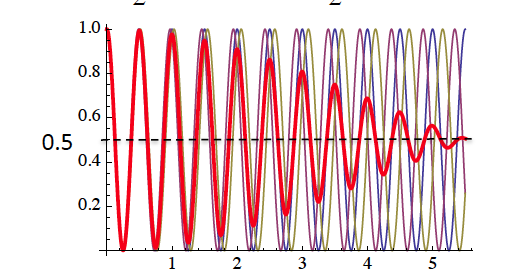
\includegraphics[height=4cm]{deph1}
    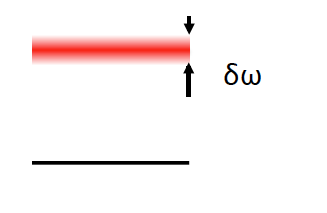
\includegraphics[height=4cm]{deph2}
  \end{figure}

  \newpage

 \subsection{Dynamics with Pauli Matrices\label{subsec:dynamics_with_pauli}}
 Summarising up to this point, we have argued for the appearance of the
 Linbland term  in the Master  equation to account for  decoherence and
 relaxation          processes          in          the          system
 \red{{\large   \begin{equation}\label{Totalequation}   \mathcal{L}   =
       \imatrixTwoColTwoRow{\Gamma_1\rho_{11}                         -
         \Gamma^{ex}\rho_{00}}{-\Gamma_2\rho_{01}}{-\Gamma_2\rho_{10}}{\Gamma^{ex}\rho_{00}-\Gamma_1\rho_{11}};\quad
       \dot{\rho}                                                     =
       -\frac{i}{\hbar}\big[\mathcal{H},\rho\big]+\mathcal{L},
     \end{equation}}}

 \noindent and shown a few useful expectation values, that allow one to
 express the dynamics  of the system via the expectation  values of the
 Pauli matrices, Eq.\eqref{expectation}

 \red{{\large           \begin{equation}          \rho_{00}           =
       \frac{\iaverage{\sigma_z}+1}{2};\quad
       \rho_{01}=\frac{\iaverage{\sigma_x}-i\iaverage{\sigma_y}}{2}   =
       \iaverage{\sigma_{+}};\quad\rho_{10}=\frac{\iaverage{\sigma_x}+i\iaverage{\sigma_y}}{2}
       =             \iaverage{\sigma_{-}};\quad\rho_{11}             =
       \frac{1-\iaverage{\sigma_z}}{2}.
     \end{equation}
     \begin{equation}
       \iaverage{\sigma_x}=\rho_{01}+\rho_{10};\quad\iaverage{\sigma_y} = i\rho_{01}-i\rho_{10};\quad\iaverage{\sigma_z}=\rho_{00}-\rho_{11}
     \end{equation}}}

 \noindent Lets compute the evolution of these expectation values

 \begin{equation}\label{evolution}
   \begin{aligned}
     \frac{d\iaverage{\sigma_j}}{dt} & =\itrace{\sigma_j\frac{d\rho}{dt}} = \itrace{-\frac{i}{\hbar}\sigma_j\big(\mathcal{H}\rho - \rho\mathcal{H}\big)+\sigma_j\mathcal{L}}\\
     \mathcal{H}                           &                          =
     \frac{\hbar\Omega}{2}\bigg(\sigma_x\cos(\phi)-\sigma_y\sin(\phi)\bigg),
   \end{aligned}
 \end{equation}

 \noindent and evaluating for all the matrices

 \begin{equation}\label{pauliDeriv}
   \begin{aligned}
     \frac{d\iaverage{\sigma_x}}{dt}&=-i\frac{\Omega}{2}\itrace{\big(\sigma_x\sigma_x\rho-\sigma_x\rho\sigma_x\big)\cos(\phi) + \big(\sigma_x\sigma_y\rho-\sigma_x\rho\sigma_y\big)\sin(\phi)} + \itrace{\sigma_x\mathcal{L}}\\
     & = \Omega\iaverage{\sigma_z}\sin(\phi)-\Gamma_2\iaverage{\sigma_x}\\
     \frac{d\iaverage{\sigma_y}}{dt}& = \Omega\iaverage{\sigma_z}\sin(\phi)-\Gamma_2\iaverage{\sigma_y}\\
     \frac{d\iaverage{\sigma_y}}{dt}& = -\Omega\big(\iaverage{\sigma_x}\cos(\phi)+\iaverage{\sigma_y}\sin(\phi)\big)-\Gamma_1\iaverage{\sigma_z}+\Gamma_1\\
   \end{aligned}
 \end{equation}

 \noindent or in more compact form

  \begin{equation}\label{pauliEv}
    \frac{d}{dt}\begin{pmatrix}
      \iaverage{\sigma_x}\\\iaverage{\sigma_y}\\\iaverage{\sigma_z}
    \end{pmatrix} = \begin{pmatrix}
      -\Gamma_2 & 0 & \Omega\sin(\phi) \\ 0 &-\Gamma_2 & \Omega\cos(\phi) \\ -\Omega\sin(\phi) & -\Omega\cos(\phi) & -\Gamma_1\\
    \end{pmatrix}\begin{pmatrix}
      \iaverage{\sigma_x} \\ \iaverage{\sigma_y} \\ \iaverage{\sigma_z}
    \end{pmatrix} + \begin{pmatrix} 0\\0\\\Gamma_1
    \end{pmatrix}    \rightarrow     \red{    \frac{d\vec{\iaverage{\sigma}}}{dt}    =
      B\vec{\iaverage{\sigma}}+\vec{b}.  }
  \end{equation}

  \noindent The  dynamics of this  system are the  exact same as  for a
  spin 1/2 particle  in a magnetic field \textbf{B}  studied in Chapter
  \ref{spin12}    Eq.~\eqref{eqn:evolutionBloch}.      The    different
  components of  the vector \isigma can  be plotted on a  sphere.  Note
  that  unlike  the Bloch  sphere  used  previously, these  vectors  do
  \textbf{not}  have  to  be  on   the  surface.   The  various  states
  $ \vec{\iaverage{\sigma}} $ correspond to

  \begin{align}
    \rho_{00}=1 & \rightarrow \isigma = \imatrixThreeCol{0}{0}{1}\\
    \rho_{11}=1 & \rightarrow \isigma = \imatrixThreeCol{0}{0}{-1}\\
    \rho_{00}=\rho_{11}&\rightarrow\isigma = \imatrixThreeCol{\cos(\phi)}{\sin(\phi)}{0}
  \end{align}

  \begin{figure}[h]
    \centering 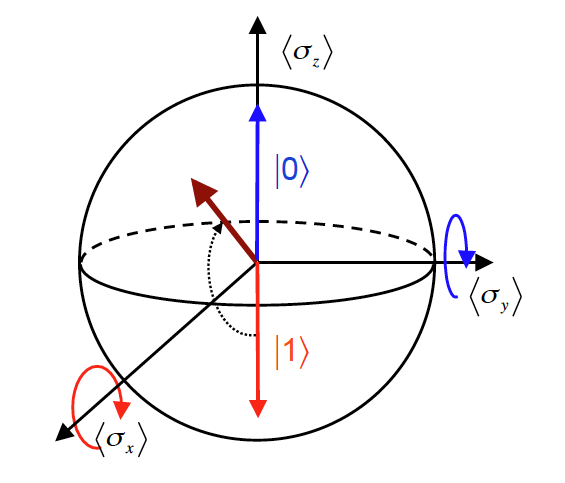
\includegraphics[height=7cm]{sphere}
  \end{figure}

  \newpage

  \paragraph{Starting in the superposed state}

  So now let  us study some dynamics, where, unless  specified, we take
  the initial state to be $  \rho_{00}=1/2 $ i.e.  on the equator where
  the atom  has equal  occupation in levels  \iket{0} and  \iket{1}. An
  general state would be

 \[
   \Psi   =  \frac{\iket{0}+e^{i\phi}\iket{1}}{\sqrt{2}}   \quad  \rightarrow   \quad  \rho   =
   \frac{1}{2}\imatrixfour{1}{e^{-i\phi}}{e^{i\phi}}{1}
 \]

 \begin{itemize}
 \item \textbf{\red{No driving} No  decoherence} - the superposed state
   will remain superposed.
   \[
     \begin{aligned}
       \mathcal{H} = -\frac{\hbar\omega}{2}\sigma_z &\iRa  U = \imatrixfour{e^{i\omega t}}{0}{0}{e^{-i\omega t}}\\
       &\iRa \rho(t) = U\rho(0)U\idagger = \frac{1}{2}\imatrixfour{e^{i\omega t}}{e^{i(\omega t - \phi)}}{e^{-i(\omega t - \phi)}}{e^{-i\omega t}}\imatrixfour{e^{-i\omega t}}{0}{0}{e^{+i\omega t}}\\
       &\qquad                                 \qquad\qquad\qquad\red{=
         \frac{1}{2}\imatrixfour{1}{e^{i(2\omega t - \phi)}}{e^{-i(2\omega
             t - \phi)}}{1}}
     \end{aligned}
   \]

   \red{But  when  we  consider  the situation  from  by  entering  the
     rotating     frame     (the      interaction     picture),     see
     Chapter~\ref{sec:unitary} and Ch.~\ref{sec:interaction}}

  \[
    U_0(t) = e^{i\frac{\mathcal{H}_0}{\hbar}t},
  \]

  \noindent the  interaction picture  Hamiltonian will  be of  the form
  Eq.~\eqref{eqn:interactionPictureHamiltonian}

  \[
    \mathcal{H}_i       =       U_0(t)\idagger\bigg[\mathcal{H}       -
    \mathcal{H}_0\bigg]U_0(t) \equiv 0,
  \]

  \noindent and  so there will  be no evolution  in the system  in this
  rotated frame that  we work with.  The  expectation values, \isigmax,
  \isigmaz are the same as in the rotated and non-rotating frames:

  \begin{equation}
    _I\bra{\psi}\hat{O}_I\ket{\psi}_I = _S\bra{\psi}U_0U_0^\dagger\hat{O}_SU_0U_0^\dagger\ket{\psi}_s \equiv _S\bra{\psi}\hat{O}_S\ket{\psi}_S
  \end{equation}

\begin{figure}[h]
  \centering 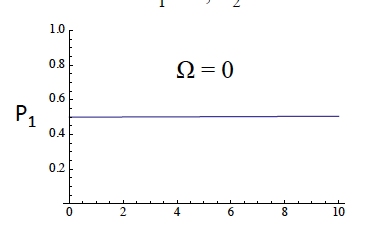
\includegraphics[height=4cm]{doD2}
\end{figure}

\begin{figure}[h]
  \centering 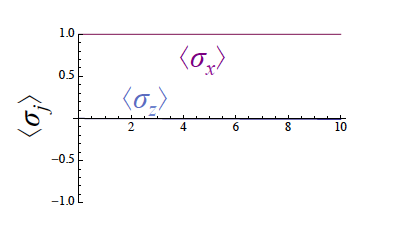
\includegraphics[height=4cm]{doD1}
  \caption{\small }
\end{figure}

  \begin{figure}[h]
    \centering 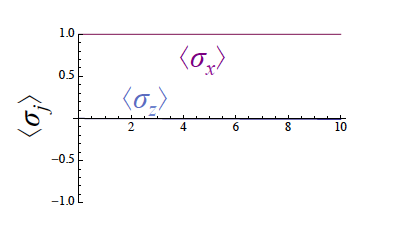
\includegraphics[height=4cm]{doD1}
    \caption{\small  On  the  equator  the atom  has  equal  weight  in
      \iket{0}  and  \iket{1},  so  \isigmaz is  0.   The  \isigmax  is
      stationary.}
  \end{figure}

  \newpage
\item          \textbf{\red{Driving}           No          decoherence,
    $ \Gamma_1 = 0, \Gamma_2 = 0 $}

  We evolution  of the wavefunction is  taken to be \red{under  a drive
    from a resonant field}

  \begin{equation}\label{dunamicState}
    \ket{\Psi} = \cos\left(\frac{\Omega t}{2}\right)\ket{0} + i\sin\left(\frac{\Omega t}{2}\right)\ket{1}; \quad \rho = \iketbra{\Psi}{\Psi}
  \end{equation}


  \begin{equation}\label{dyn1}
    \begin{aligned}
      \rho_{11} & = \sin^2(\Omega t/2) & \iaverage{\sigma_x} & = \rho_{01}+\rho_{10} = \sin(\Omega t)\\
      \rho_{01} & = \sin(\Omega t/2)\sin(\Omega t/2) = \frac{\sin(\Omega t)}{2} & \iaverage{\sigma_y} & = i\rho_{01}-i\rho_{10} = 0\\
      \rho_{10} & = \sin(\Omega t/2)\sin(\Omega t/2) = \frac{\sin(\Omega t)}{2} & \iaverage{\sigma_z} & = 1- 2\rho_{00} = \cos(\Omega t)\\
    \end{aligned}
  \end{equation}

  \noindent  and the  point  on  the sphere  simply  rotates about  the
  \iaverage{\sigma_y} axis.  If there was  a phase shift in the driving
  field $  \phi $  then the rotation  would turn by  that angle  about the
  \iaverage{\sigma_z} axis. Overall these are the Rabi oscillations

  \begin{figure}[h]
    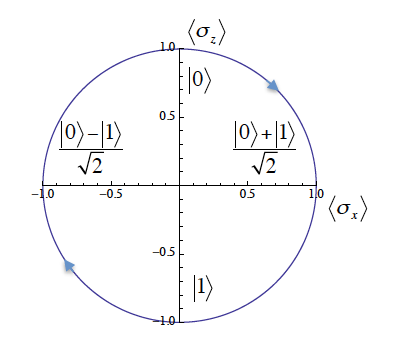
\includegraphics[height=4cm]{dyn1}
    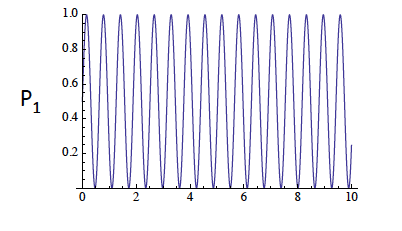
\includegraphics[height=4cm]{dnO}
  \end{figure}

  \newpage
\item       \textbf{\textbf{\red{Driving}        With       decoherence
      $ \Gamma_1 =  1, \Gamma_2 = 0.5, \gamma =  \Gamma_1+\Gamma_2/2 $}}, it
  is  simpler   to  solve   the  dynamics  of   Eq.\eqref{pauliEv}  for
  \iaverage{\vec{\sigma}}

  For the case when one starts off with state $ \rho_{00} = 1 $

  \begin{equation}\label{dyn2}
    \begin{aligned}
      \iaverage{\sigma_x} & \approx e^{-\gamma t} \sin(\Omega t) & \rho_{00} & = \frac{\iaverage{\sigma_z}+1}{2} \approx\frac{1+e^{-\gamma t} \cos(\Omega t)}{2}\\
      \iaverage{\sigma_y} & = 0 & \rho_{01} & = \frac{\iaverage{\sigma_x}-i\iaverage{\sigma_y}}{2} = \frac{e^{-\gamma t} \sin(\Omega t)}{2}\\
      \iaverage{\sigma_z} & \approx e^{-\gamma t} \cos(\Omega t) & \rho_{10} & = \frac{\iaverage{\sigma_x}+i\iaverage{\sigma_y}}{2} = \frac{e^{-\gamma t} \sin(\Omega t)}{2}\\
    \end{aligned}
  \end{equation}

  \noindent In  this case the  two components begin  to spiral in  as a
  result  of  the  dephasing.   The central  point  is  the  stationary
  condition in  which both \iaverage{\sigma_x}  and \iaverage{\sigma_z}
  take on a finite value - the stationary state value.

   \begin{figure}[h]
     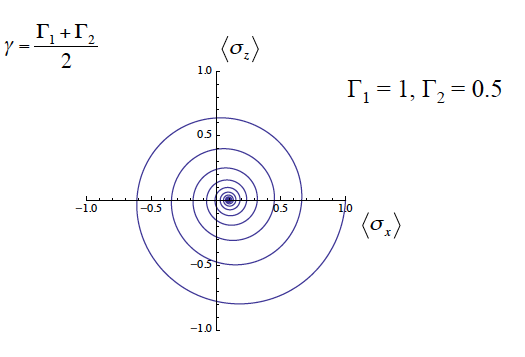
\includegraphics[height=6cm]{dyn2}
     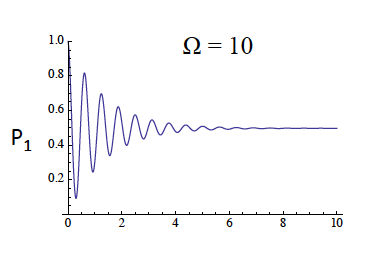
\includegraphics[height=5cm]{dd}
   \end{figure}

   \newpage
 \item  \textbf{\red{No  driving}   with  decoherence  and  relaxation}
   $ \rho_{00}=\rho_{11} = 1/2 $ then

   \begin{equation}\label{dyn21}
     \begin{aligned}
       \iaverage{\sigma_x} & = e^{-\Gamma_2 t} & \rho_{00} & = 1-\frac{e^{-\Gamma_1 t}}{2}\\
       \iaverage{\sigma_y} & = 0 & \rho_{01} & = \frac{e^{-\Gamma_2 t}}{2} \\
       \iaverage{\sigma_z} & = 1 - e^{-\Gamma_1 t} & \rho_{10} & = \frac{e^{-\Gamma_2 t}}{2} \\
     \end{aligned}
   \end{equation}

   The system, initially on the `equator' of the sphere, transitions to
   the ground state

     \begin{figure}[h]
       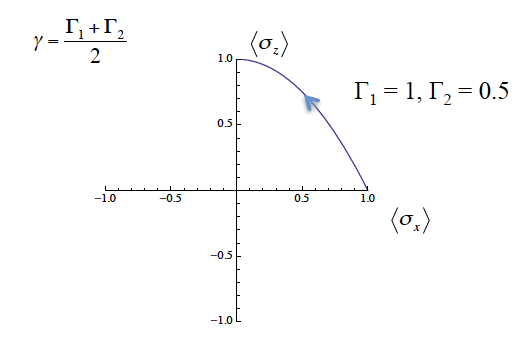
\includegraphics[height=6cm]{dyn21}
       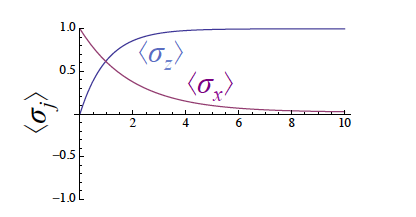
\includegraphics[height=6cm]{dyn22}
     \end{figure}

   \item       \textbf{\red{No       driving}      Only       dephasing
       $ \Gamma_1=0, \Gamma_2 \ne 0 $}  when we start off in a superposed
     state $ \rho_{11}=1/2\rightarrow\iaverage{\sigma_z}=0 $

     \begin{equation}\label{dyn3}
       \begin{aligned}
         \iaverage{\sigma_x} & = e^{-\Gamma_2 t} & \rho_{00} & = \frac{1}{2}\\
         \iaverage{\sigma_y} & = 0 & \rho_{01} & = \frac{e^{-\Gamma_2 t}}{2} \\
         \iaverage{\sigma_z} & = 0 & \rho_{10} & = \frac{e^{-\Gamma_2 t}}{2} \\
       \end{aligned}
     \end{equation}

     The  expectation  value simply  moves  towards  the origin,  where
     $ \iaverage{\sigma_z} = 0 $  and the system becomes equally likely
     to  exist in  the excited  or ground  state $  \rho_{00}=\rho_{11}
     $. The off diagonal terms loose coherence.

   \begin{figure}[h]
     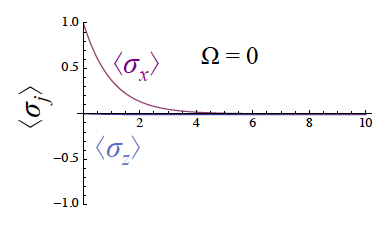
\includegraphics[height=6cm]{dyn31}
     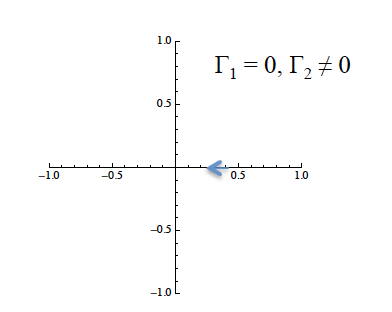
\includegraphics[height=4cm]{nd1}
   \end{figure}
 \end{itemize}

 {\large   \red{\textbf{Thus,    relaxation   will   tend    to   shift
       \iaverage{\sigma_z} to  1, and  together with pure  dephasing it
       shortens the  expectation values of the  \iaverage{\sigma_x} and
       \iaverage{\sigma_y} directions.}}}
 \newpage
